

\chapter{Puzzles, Algorithms \& Hardness} 


\label{ch:puzz-algo-hard}
\section{Coloring Puzzle}

\begin{figure}[h] \label{fig:graph}
\centering 
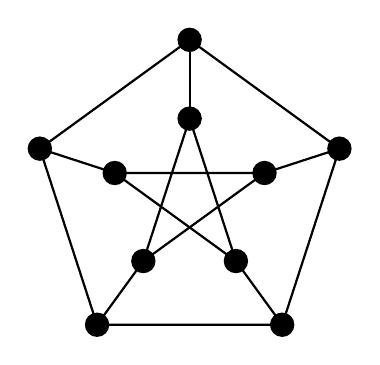
\begin{tikzpicture}[style=thick] 
\draw (18:2cm) -- (90:2cm) -- (162:2cm) -- (234:2cm) -- (306:2cm) -- cycle;
\draw (18:1cm) -- (162:1cm) -- (306:1cm) -- (90:1cm) -- (234:1cm) -- cycle;
\foreach \x in {18,90,162,234,306}{ 
	\draw (\x:1cm) -- (\x:2cm); 
}
\draw[fill=black] (18:2cm) circle (4pt);
\draw[fill=black] (90:2cm) circle (4pt);
\draw[fill=black] (90:1cm) circle (4pt); 
\draw[fill=black] (18:1cm) circle (4pt); 
\draw[fill=black] (162:1cm) circle (4pt); 
\draw[fill=black] (162:2cm) circle (4pt); 
\draw[fill=black] (234:1cm) circle (4pt);
\draw[fill=black] (234:2cm) circle (4pt); 
\draw[fill=black] (306:1cm) circle (4pt); 
\draw[fill=black] (306:2cm) circle (4pt);
\end{tikzpicture} 
\end{figure}

Consider the following puzzle. Given a figure
as above, the goal is to give colors to the circles such that
for every line, its end points have different colors. Furthermore, the number of
colors used needs to be minimized. Without this condition the problem is
trivial since using a different color for every circle would be a solution
irrespective of the figure.

Puzzles like above are very commonly encountered in a variety of real life
instances. However known algorithms takes far too much time to complete even on
instances with $20$ vertices. This thesis is about an explanation for the
lack of efficient algorithms, for coloring like problems.

\begin{figure}[h] 
\centering 
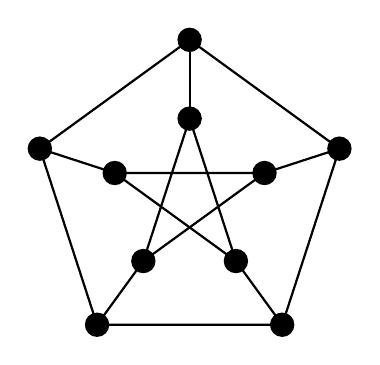
\begin{tikzpicture}[style=thick] 
\draw (18:2cm) -- (90:2cm) -- (162:2cm) -- (234:2cm) -- (306:2cm) -- cycle;
\draw (18:1cm) -- (162:1cm) -- (306:1cm) -- (90:1cm) -- (234:1cm) -- cycle; 
\foreach \x in {18,90,162,234,306}{ \draw (\x:1cm) -- (\x:2cm); }
\draw[fill=black] (18:2cm) circle (4pt); 
\draw[fill=black] (90:2cm) circle (4pt); 
\draw[fill=black] (90:1cm) circle (4pt); 
\draw[fill=black] (18:1cm) circle (4pt); 
\draw[fill=black] (162:1cm) circle (4pt); 
\draw[fill=black] (162:2cm) circle (4pt); 
\draw[fill=black] (234:1cm) circle (4pt);
\draw[fill=black] (234:2cm) circle (4pt); 
\draw[fill=black] (306:1cm) circle (4pt); 
\draw[fill=black] (306:2cm) circle (4pt);
\end{tikzpicture} 
\qquad \qquad  
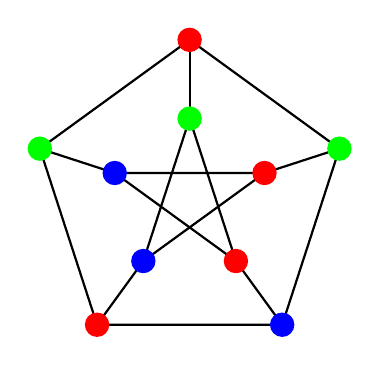
\begin{tikzpicture}[style=thick] 
\draw (18:2cm) -- (90:2cm) -- (162:2cm) -- (234:2cm) -- (306:2cm) -- cycle; 
\draw (18:1cm) -- (162:1cm) -- (306:1cm) -- (90:1cm) -- (234:1cm) -- cycle; 
\foreach \x in {18,90,162,234,306}{ 
	\draw (\x:1cm) -- (\x:2cm); 
}
\draw[color=green,fill=green] (18:2cm) circle (4pt); 
\draw[color=red,fill=red] (90:2cm) circle (4pt); 
\draw[color=green,fill=green] (90:1cm) circle (4pt);
\draw[color=red,fill=red] (18:1cm) circle (4pt); 
\draw[color=blue,fill=blue] (162:1cm) circle (4pt); 
\draw[color=green,fill=green] (162:2cm) circle (4pt);
\draw[color=blue,fill=blue] (234:1cm) circle (4pt); 
\draw[color=red,fill=red] (234:2cm) circle (4pt); 
\draw[color=red,fill=red] (306:1cm) circle (4pt);
\draw[color=blue,fill=blue] (306:2cm) circle (4pt); 
\end{tikzpicture}
\caption{The figure on the right is a $3$-coloring of the graph on the left.
However it does not have a $2$-coloring.} 
\label{fig:M1} 
\end{figure} 
Figures
like above are commonly called \emph{graphs}
 (strictly speaking they are undirected graphs, but in this thesis will
 only be concerned with undirected graphs) . A graph $G=(V,E)$ consists of a
set of \emph{vertices} $V$ (the circles) and a set $E$ containing some pairs of
vertices, called \emph{edges} (the lines).

Given a graph $G=(V,E)$ and a number $C$, a $C$-coloring of $G$ is an assignment
of \emph{colors} denoted by $\{1,\cdots, C\}$ to the vertices such that the end
points of every edge have different colors. For a given graph, a $C$-coloring
might not exist for all values of $C$. But for any graph, the coloring which
gives different colors to all vertices in $V$, is an $n$-coloring, where $n$ is
the \emph{size} (the number of vertices in $V$) of $G$.

\begin{definition} The \GraphColoring\ problem is, given a graph, find a
coloring, using the minimum number of colors. This
minimum value is commonly known as the \emph{chromatic number} of the graph.
\end{definition}

\section{Efficient Algorithms}

If the maximum degree of $G$ is $\Delta$ then the following simple algorithm computes
a $(\Delta+1)$-coloring in time bounded by the number of edges.
\paragraph{}
\begin{algorithm}[H] 
\caption{For graphs with maximum degree $\leq\Delta$.} 
\For{$v \in V$}{ 
	give $v$ a color in $\{1,\cdots,\Delta+1\}$ different from the colors of its
	already colored neighbours.
} 
\end{algorithm}
\qquad

Algorithm 1, does not solve the \GraphColoring\ problem since the chromatic
number can be much smaller than $\Delta+1$.
Suppose the graph has a $c$-coloring there is a simple algorithm to find it,
which takes $c^n\cdot m$ time, where $m$ is the number of edges.
\paragraph{}
\begin{algorithm}[H] 
\label{alg:brut} 
\caption{Brute Force Algorithm} 
\For{every assignment $f \in \{1,\cdots,c\}^V$ of colors to the vertices }{ 
	\For{every edge}{
		check if $f$ assigns different colors to the end points.
	} 
}
\end{algorithm}
\qquad

However note that the running time of Algorithm 2 grows
\emph{exponentially} in $n$. Even for $n=20$, the running time ($> c^{20}$) is
prohibitively large, while for Algorithm 1 it is still a reasonable number. This
motivates the definition of efficient algorithms, as ones that has running time
bounded by a polynomial in the input size. For simplicity, we consider only
\emph{decision problems} (\ie problems that have a Boolean answer). For such
problems the inputs are partitioned into YES and NO instances. We will often
specify a decision problem by the set of YES instances. Though \GraphColoring\
problem is not a decision problem, we can consider the problem which have the
number $C$ also in the input, where the goal is to check if the graph has a
$C$-coloring. 
%TODO: Motivate and give references for efficient = polytime

\begin{informal-definition}\label{def:p} 
\P\ is the class of decision problems, that has an algorithm
with running time bounded by a polynomial in $n$ (the input size).
\end{informal-definition}

Note that for \GraphColoring, $(G,C) \in \YES$ (i.e. $G$ has a $C$-coloring),
then there is a certificate that certifies that it is \YES\ instance, that can
be verified in time proportional to the number of edges. The certificate is
simply the $C$-coloring of the graph. And if $(G,C) \in \NO$, then any assignment
of colors from $\{1,\cdots, C\}$, will leave some edge monochromatic. This
property is true for a large class of problems.

\begin{informal-definition} \label{def:np}
 \NP\ is the class of decision problems, for which there is an
algorithm $V$ which takes an input $x$ and a proof $\pi$, runs in time
polynomial in the size of $x$ and satisfies the following properties.
\begin{itemize} 
\item Completeness : If $x \in \YES$ then there exists $\pi$
such that $V(x,\pi)=1$. 
\item Soundness : If $x\in \NO$ then for any $\pi$,
$V(x, \pi)=0$. 
\end{itemize} 
\end{informal-definition}

For any \NP\ problem, there is a trivial algorithm similar to Algorithm
\ref{alg:brut}, which runs in time $c^n$ for some constant $c$. The algorithm
just tries all possible certificates with the verification procedure. It is a
major open problem if \P $=$ \NP. A surprising result is that there are certain
class of problems called \NPComplete\ which capture the hardness of solving
problems in \NP. That is, an instance of any \NP\ problem could be converted
efficiently to an instance of such problems. 
The \GraphColoring\ problem is an \NPComplete\ problem. Hence unless $\P = \NP$,
we cannot hope to have polynomial time algorithms for \GraphColoring. One can
ask if there are polynomial time algorithms for a relaxed version of the
problem.

\section{Approximation Algorithms} 
\label{sec:approx} 
A relaxed
version of the \GraphColoring\ problem is to compute the chromatic number
approximately. An \emph{approximation algorithm} for chromatic number with
approximation \emph{factor} $F \geq 1$, always outputs a number between $C$ and
$C\cdot F$, where $C$ is the chromatic number of the input graph.
 
However for a general graph, this relaxation is also a \emph{hard} problem. That
is, assuming the famous $\P\neq \NP$ conjecture, it is known that this problem
cannot be solved in polynomial time. Feige \& Kilian~\cite{FeigeK00} showed that
computing this number approximately within a factor of $n^{1-\epsilon}$ for any
small constant $\epsilon >0$ is known to be  hard, assuming a different complexity
conjecture. Therefore, there is not much hope of having an efficient algorithm,
which does much better than the trivial $n$-coloring.

Since the general approximation problem is hard, the focus shifted on solving it
for subclasses of graphs. A natural subclass of graphs to consider, are the ones
for which the chromatic number is a small constant $c$. For $c=2$, such graphs
are commonly called \emph{bipartite}. There is a simple linear time algorithm
for finding a $2$-coloring in such graphs. It just assigns a vertex one color,
the other color to all its neighbours, and continues until all vertices are
colored. However for $3$-colorable graphs, finding a $3$-coloring is \NPHard\
(it cannot be solved by efficient algorithms, assuming \P$\neq$ \NP).

Hence a long series of works, was aimed at solving this problem approximately.
\begin{definition} 
\ApproximateGraphColoring$(c,C)$ problem is to find a
$C$-coloring, when the input graph is promised to be $c$-colorable.
\end{definition} 

\begin{remark}
We will often be considering the decision version of the problem, specified by
disjoint sets of \YES\ ($c$-colorable graphs) and \NO\ (graphs with chromatic
number $> C$) instances. The goal is to have an algorithm to accept all \YES\
instances and reject all \NO\ instances. The algorithm can either accept 
or reject inputs which are neither \YES\ nor \NO. 
\end{remark}

For $3$-colorable
graphs, Wigderson~\cite{Wigderson83} gave the first not trivial improvement of
finding a $O(\sqrt n)$-coloring using combinatorial techniques. This was further
improved to $O(n^{3/8})$-coloring by Blum~\cite{Blum94}. A major breakthrough
 was made by Karger, Motwani \&
Sudan~\cite{KargerMS1998}, using semi-definite programming (SDP). For a
$3$-colorable graph with maximum degree $d$, they gave an $O(d^{1/3})$-coloring
algorithm. Combining this with Wigderson's algorithm, they obtained a
$O(n^{1/4})$-coloring algorithm. Blum \& Karger~\cite{BlumK1997} combined the
combinatorial methods of Blum~\cite{Blum94} with the SDP to get an
$O(n^{3/14})$-coloring. The current best known (see results of Kawarabayashi \& Thorup
\cite{KawarabayashiT2014}) efficient algorithms output a $n^{0.19996}$-coloring.


\section{What this thesis is about?}

This thesis is about giving an explanation for the lack of efficient algorithms for
some generalizations of the \ApproximateGraphColoring$(c,C)$ problem, 
using the theory of \NPComplete ness and complexity conjectures similar 
to \P $\neq$ \NP. That is, we prove that efficient algorithms for the problem
will imply that the corresponding conjecture is false.  
Such results are called \emph{hardness 
results} and the area in general, is commonly called in literature as
the \emph{hardness of approximation}. The focus of our hardness
results will be the case when $c$ is a small constant and $C$ can be 
any large constant or a function that depends on $n$. 
As described in the previous section,
there are algorithms which solve these problems for $C=n^\alpha$ for
some constant $\alpha <1$. We prove hardness results for larger values
(exponentially larger in some cases)
of $C$ than was previously known. 
We will describe these generalizations in the next three sections.

\subsection{Almost Coloring}

Assuming \P$\neq$ \NP, Khanna \etal~\cite{KhannaLS2000}
showed hardness for the \ApproximateGraphColoring$(3,4)$ problem
 (that is there is no efficient algorithm which can find a $4$-coloring,
 in any $3$-colorable graph). Since then, there has been no progress
 in  this problem. Later, results where proved using a complexity
  assumption called the Unique Games Conjecture (UGC), 
  which is stronger than the P$\neq$ NP assumption.
Starting with the work of Khot~\cite{Khot2002}, it was shown that  
UGC, explains the lack of efficient approximation algorithms for a 
variety of problems (eg. Vertex Cover, MAX-CUT).
 Dinur, Mossel \& Regev~\cite{DinurMR2009} showed hardness for
 \ApproximateGraphColoring$(3,C)$ for any constant $C$ using
 a conjecture similar to \UGC. Due to a technical problem (that
 \UGC\ does not have perfect completeness), their results which
 used \UGC\ exactly, showed hardness for the 
 \AlmostGraphColoring{\epsilon}$(c,C)$ problem, for any small
 $\epsilon >0$.
 \begin{definition}
 The \AlmostGraphColoring{\epsilon}$(c,C)$ problem is
 of distiguishing graph from the following cases:
 \begin{itemize}
 \item \YES\ : There is a subgraph of size $(1-\epsilon)n$ that is 
 $c$-colorable.
 \item \NO\ : Any independent set is the graph has size at most $n/C$.
 \end{itemize}
 \end{definition}
 \noindent
 \paragraph{\underline{Contributions of this Thesis:}}	
The work of Dinur \& Shinkar~\cite{DinurS2010} 
implies hardness results for \AlmostGraphColoring{\epsilon}$(3,\poly(\log n))$,
 using a stronger form of \UGC\ (where the dependence
 between the soundness and alphabet size is inverse polynomial).
In \lref[Chapter]{ch:graph-hard}, we show hardness for 
the same problem, using a weaker form of UGC (in which the 
aforesaid dependence 
is super-polynomial) in some respects (joint work with Dinur, Harsha \& Srinivasan~\cite{DinurHSV2014}).

The previous reductions (by Dinur, Mossel \& Regev~\cite{DinurMR2009}
and Dinur \& Shinkar~\cite{DinurS2010}) followed
the template of H\aa stad \cite{Hastad2001}, which employed a particular
error correcting code known as the long code. As the name implies, this
code has a large size which made the reductions inefficient. A shorter
code called the low degree long code was proposed by 
Barak \etal~\cite{BarakGHMRS2012} . Dinur and Guruswami~\cite{DinurG2013} showed
improved approximate covering (which we define in \lref[Section]{sec:intro-cover}) hardness results 
 using this shorter code. In \lref[Chapter]{ch:graph-hard}, we  adapt this shorter code
  to the reduction of Dinur, Mossel and Regev~\cite{DinurMR2009} for graph coloring,
  to get improved results.
 
 

 
  %Mention results of Sion Chan, Sanxia Huang, Khot, DinurMR, DS on graph coloring hardness
 

\subsection{Hypergraph Coloring}		

Guruswami, H\aa stad \& Sudan~\cite{GuruswamiHS2002} initiated
the study of hypergraph coloring problems, to
get a better understanding of graph coloring and since it
is a natural generalization. They showed
hardness results for $c=2, C=\poly(\log \log n)$, for hypergraph coloring, 
assuming
that \NP\ does not have quasi-polynomial algorithms (such
results are commonly known as \emph{quasi-\NP-hardness} results). 
A
\emph{$k$-uniform hypergraph} $G=(V,E)$ is similar to a graph, with the edges
$E\subseteq {V \choose k}$ containing $k$ vertices. A $c$-coloring of a hypergraph is
coloring of vertices using colors $\{1,\cdots, c\}$, such that every edge
has $2$ vertices with distinct colors. For $k=2$,
a hypergraph is simply a graph. 
%TODO: Strictly speaking this is not a generalization since all vertices in an edge 
% may not be distinct. But the proofs also holds for undirected versions. 
\begin{definition} 
The \ApproximateHypergraphColoring{k}$(c,C)$ problem is defined similar to
\ApproximateGraphColoring$(c,C)$, as given a $c$-colorable $k$-uniform
hypergraph, find a $C$-coloring. The decision version is also defined
analogously. 
\end{definition}
When $k>2$, for any constant $c>1$, known algorithms only guarantee an
 $n^\alpha$-coloring for some $\alpha < 1$. Starting
 with the work of Guruswami, H\aa stad \& Sudan \cite{GuruswamiHS2002}, 
 there have been many results in hardness of hypergraph coloring.
 For the case of constant $c,k$, strongest known results 
 due to Khot~\cite{Khot2002c}, who showed 
quasi-\NP-hardness  for $C= \poly( \log n)$.
\noindent
\paragraph{\underline{Contributions of this Thesis:}}
In \lref[Chapter]{ch:hypergraph-hard}, we exponentially improve the hardness
results.  In \lref[Section]{sec:33}, we first show hardness results (joint work with Guruswami, Harsha, H\aa stad \& 
Srinivasan~\cite{GuruswamiHHSV2014}) for 
$3$-uniform $3$-colorable hypergraphs by a more efficient reduction,
that makes use of low degree long code (which we describe in \lref[Section]{sec:low-deg-long-code}).
For the case of $4$-uniform $4$-colorable hypergraphs, 
our initial work (joint work with Guruswami, Harsha, H\aa stad \& 
Srinivasan~\cite{GuruswamiHHSV2014}) showed the first
super-polylogarithmic coloring hardness (i.e. $C >> \poly(\log n)$)  results, by
using the low degree long code. 
Subsequent to our initial work Khot \&
Saket~\cite{KhotS2014b} got hardness results of $2^{(\log
n)^{1/21}}$, by using the low degree long code with degree $2$. Though their result was
for $12$-uniform hypergraphs. We further observed~\cite{Varma2014} that
by combining their methods with ours, the same hardness results can be
obtained for $4$-uniform hypergraphs. Hence  we improved the hardness
results from $\poly(\log n)$ to $2^{(\log n)^{1/21}}$ for
the case of $4$-colorable $4$-uniform hypergraphs. 

\subsection{Covering CSPs}
\label{sec:intro-cover}
The covering problem for constraint satisfaction~(CSP) is a generalization of the hypergraph
coloring problem, introduced by
Guruswami, H\aa stad and Sudan~\cite{GuruswamiHS2002} and later studied in 
detail by Dinur \& Kol~\cite{DinurK2013}. An instance of the problem
consists of a hypergraph $G=(V,E)$ along with a \emph{predicate} $P
\subseteq \{0,1\}^k$ and a \emph{literal} function $L:E\rightarrow
\{0,1\}^k$. An \emph{assignment} $f:V \rightarrow \{0,1\}$
\emph{covers} an edge $e\in E$, if $f|_e \oplus L(e) \in P$ (by $f|_e$,
we mean the $k$ bit string, obtained by restricting $f$ to vertices in $e$, and the 
$\oplus$ operation is coordinate-wise parity of the two strings). 
A \emph{cover} for a CSP instance is a set of 
assignments such that every edge is covered by one of the assignments.
 The goal of the covering problem is to find the minimum sized cover.
 
 When the predicate is the $3$-OR predicate, we can view the
 instance as a $3$-SAT instance, where each edge is a clause and the literal function
 specifies which variables are to be negated.
 Then the satisfiability problem is equivalent to finding a cover of size $1$.
The covering problem can also be thought of as a generalization of the coloring
problem. Consider an instance $G$  with the NAE(
$:=\{0,1\}^k \setminus \{ \overline 0, \overline 1\}$) predicate 
and the trivial literal function $L(e) = 0^k$ for every edge $e$.
It is not difficult to see that $G$ has a cover of size $t$
 iff $G$ is $2^t$-colorable. The \emph{approximate covering} problem is defined as,
given a $c$-coverable instance, find a $C$-covering.\\
\begin{definition}[\cov-$P$-\csp$(c,C)$]
  
	\label{def:cov-csp}
	For $P \subseteq \setq^k$ and $c,C \in \nat$, the \cov-$P$-\csp$(c,C)$ problem is, 
	given a $c$-coverable instance  $(G=(V,E),L)$ of $P$-\csp, find an 
	$C$-covering.
\end{definition}

A predicate $P$ is \emph{odd}, if for every $x \in \{0,1\}^k$ either $x \in
P$ or $\overline{x} \in P$. For odd predicates,
there is a trivial algorithm with factor $2$, since any assignment
and its complement covers the CSP instance. Dinur \& Kol~\cite{DinurK2013} asked the question
whether,  the approximate covering problem is hard for any constant $C>c$, for all non-odd
predicates. Assuming a variant of UGC, they proceeded to show that if a non-odd predicate has a
pairwise independent distribution in its support then, this is indeed
the case.


\noindent
\paragraph{\underline{Contributions of this Thesis:}}
In \lref[Chapter]{ch:covering-hard}, we answer the question of Dinur \& Kol in the affirmative 
(joint work with Bhangale \& Harsha~\cite{BhangaleHV2014}). That is,
the approximate covering problem for a non-odd predicate is hard for any constant $C>c$ 
(assuming the same conjecture as Dinur \& Kol used). 
This leads to a complete characterization of predicates for which this result can be true,
since there is a trivial $2$-covering algorithm for odd predicates. 
Our results also holds over non binary alphabets. 
We also show NP-hardness results, for the approximate covering problem with parameters
$c=2, C = \log \log n$, for a class of predicates. Previously such results were  known due to
Dinur \& Kol  for $4$-LIN with $c=2,C= \log \log \log n$.




\section{Organization of Thesis} 

This thesis has two main parts. In
\lref[Part]{part:two}, we will introduce some of the mathematical techniques
used in proving the hardness results. \lref[Part]{part:three} contains all the
hardness results.

In \lref[Part]{part:two}, we also prove some lemmas which form the
basis of the results in the next part. In \lref[Chapter]{ch:harmonic}, 
\lref[Section]{sec:har-poly} is a contribution of this thesis, were we 
prove analogues of results in Boolean function analysis to functions
on subspaces. 
In \lref[Chapter]{ch:testing}, we discuss
a linear algebraic result about testing low degree polynomials.
\lref[Section]{sec:square-test} is a contribution of this thesis,
though the analysis is similar to the results of Dinur \&
Guruswami~\cite{DinurG2013} mentioned in \lref[Section]{sec:prod-test}. In
\lref[Chapter]{ch:graph-prod}, we also give some combinatorial results about
derandomized graph products. \lref[Section]{sec:derand-graph-prod} and
\lref[Section]{sec:derand-maj-stab} are contributions of this thesis
which uses the results proved in \lref[Section]{sec:square-test}.

\lref[Part]{part:three} contains all the hardness results about almost graph 
coloring (\lref[Chapter]{ch:graph-hard}; joint work with Dinur, Harsha \& Srinivasan~\cite{DinurHSV2014}), hypergraph coloring
(\lref[Chapter]{ch:hypergraph-hard}; joint work with Guruswami, Harsha, H\aa stad \& 
Srinivasan~\cite{GuruswamiHHSV2014} and the result \cite{Varma2014} ), and covering problem
(\lref[Chapter]{ch:covering-hard}; joint work with Bhangale \& Harsha~\cite{BhangaleHV2014}). These results are the main contributions of
this thesis, though much of the hardness reductions and analysis are similar to
previous works.

